%%%%(c) COPYRIGHT NOTICE%FOLDUP
%%%%(c)
%%%%(c)  This file is a portion of the source for the textbook
%%%%(c)
%%%%(c)    Numerical Methods Course Notes,
%%%%(c)    Copyright 2004-2010 by Steven E. Pav
%%%%(c)
%%%%(c)  See the file COPYING.txt for copying conditions
%%%%(c)
%%%%(c)%UNFOLD

%%throat clearing%FOLDUP
\typeout{-- quadrature.tex}
\typeout{-- N� 2004-2010 Steven E. Pav}
%UNFOLD

%%local commands%FOLDUP
%UNFOLD

\chapter{Integrals and Quadrature}

%%%%%%%%%%%%%%%%%%%%%%%%%%%%%%%%%%%%%%%%%%%%%%%
\section{The Definite Integral}%FOLDUP

Often enough the numerical analyst is presented with the challenge of finding
the definite integral of some function:
\[\int_a^b f(x) \dx.\]
In your golden years of Calculus, you learned the Fundamental Theorem of
Calculus, which claims that if $f(x)$ is continuous, and $F(x)$ is an
antiderivative of $f(x),$ then
\[\int_a^b f(x) \dx = F(b) - F(a).\]

What you might not have been told in Calculus is there are some functions for
which a closed form antiderivative does not exist or at least is not known to
humankind.  Nevertheless, you may find yourself in a situation where you have
to evaluate an integral for just such an integrand.  An approximation will have
to do.

%%%%%%%%%%%%%%%%%%%%%%%%%%%%%%%%%%%%%%%%%%%%%%%
\subsection{Upper and Lower Sums}%FOLDUP

\index{Riemann integral}%
We will review the definition of the Riemann integral of a function.
A \emph{partition} of an interval \ccinv{a}{b} is a finite, ordered
collection of nodes $x_i$:
\[a = x_0 < x_1 < x_2 < \cdots < x_n = b.\]
Given such a partition, $P,$ define the upper and lower bounds on each
subinterval \ccinv{x_j}{x_{j+1}} as follows:
\begin{align*}
m_i &= \inf \setwo{f(x)}{x_i \le x \le x_{i+1}}\\
M_i &= \sup \setwo{f(x)}{x_i \le x \le x_{i+1}}
\end{align*}

Then for this function $f$ and partition $P,$ define the upper and lower sums:
\begin{align*}
L(f,P) &= \sum_{i=0}^{n-1} m_i \Parens{x_{i+1} - x_i}\\
U(f,P) &= \sum_{i=0}^{n-1} M_i \Parens{x_{i+1} - x_i}
\end{align*}

We can interpret the upper and lower sums graphically as the sums of areas of
rectangles defined by the function $f$ and the partition $P$, as in
\figref{thesums}.

%\figref{thesums}%FOLDUP
\begin{figure}[htb!]
\centering
%\subfigure[The Lower Sum]{
\subfloat[The Lower Sum]{
	\label{fig:lower}
	\includegraphics[width=0.35\columnwidth,angle=270,clip=]{lower.eps}}
\hspace{.04in}
%\subfigure[The Upper Sum]{
\subfloat[The Upper Sum]{
	\label{fig:upper}
	\includegraphics[width=0.35\columnwidth,angle=270,clip=]{upper.eps}}
\caption{The (a) lower, and (b) upper sums of a function on a given interval
are shown.  These approximations to the integral are the sums of areas of
rectangles.  Note that the lower sums are an underestimate, and the upper sums
an overestimate of the integral.}\label{fig:thesums}
\end{figure}%UNFOLD

Notice a few things about the upper, lower sums:
\begin{compactenum}[(i)]
\item $L(f,P) \le U(f,P).$
\item If we switch to a ``better'' partition (\ie a finer one), we expect that
$L(f,\cdot)$ increases and $U(f,\cdot)$ decreases.
\end{compactenum}

The notion of integrability familiar from Calculus class (that is Riemann
Integrability) is defined in terms of the upper and lower sums.

\begin{bkdefinition}
\index{Riemann Integrable}%
A function $f$ is Riemann Integrable over interval \ccinv{a}{b} if 
\[\sup_{P} L(f,P) = \inf_{P} U(f,P),\]%
where the supremum and infimum are over all partitions of the interval
\ccinv{a}{b}.
Moreover, in case $f(x)$ is integrable, we define the integral
\[\int_{a}^{b} f(x) \dx = \inf_{P} U(f,P),\]%
\end{bkdefinition}
You may recall the following
\begin{bktheorem}%
Every continuous function on a closed bounded interval of the real line is
Riemann Integrable (on that interval).%
\end{bktheorem}

Continuity is sufficient, but not necessary.  
\begin{bkexample}%FOLDUP
Consider the \emph{Heaviside function}:\index{Heaviside function}%
\[f(x) = \left\{\begin{array}{cl} 0 & x < 0\\1 & 0 \le x\end{array}\right.\]
This function is not continuous on any interval containing $0,$ but is Riemann
Integrable on every closed bounded interval.
\end{bkexample}
%UNFOLD
\begin{bkexample}%FOLDUP
Consider the \emph{Dirichlet function}:\index{Dirichlet function}%
\[f(x) = \left\{\begin{array}{cl} 0 & x \,\text{ rational}\\1 & x \,\text{ irrational}\end{array}\right.\]
For any partition $P$ of any interval \ccinv{a}{b}, we have
$L(f,P) = 0,$ while $U(f,P) = 1,$ so 
\[\sup_{P} L(f,P) = 0 \ne 1 = \inf_{P} U(f,P),\]
so this function is \emph{not} Riemann Integrable.
\end{bkexample}
%UNFOLD

%UNFOLD
%%%%%%%%%%%%%%%%%%%%%%%%%%%%%%%%%%%%%%%%%%%%%%%
\subsection{Approximating the Integral}%FOLDUP

The definition of the integral gives a simple method of approximating an integral
$\int_a^b f(x) \dx$.  The method cuts the interval \ccinv{a}{b} into a
partition of $n$ equal subintervals $x_i = a + \frac{b-a}{n},$ for
$i=0,1,\ldots,n.$  The algorithm then has to somehow find the supremum and
infimum of $f(x)$ on each interval \ccinv{x_i}{x_{i+1}}.  
The integral is then approximated by the mean of the lower and upper sums:
\[\int_a^b f(x) \dx \approx \half \Parens{L(f,P) + U(f,P)}.\]
Because the value of the integral is between $L(f,P)$ and $U(f,P),$ this
approximation has error at most
\[\half \Parens{U(f,P) - L(f,P)}.\]

Note that in general, or for a black box function, it is usually not feasible
to find the suprema and infima of $f(x)$ on the subintervals, and thus the
lower and upper sums cannot be calculated.  However, if some information is
known about the function, it becomes easier:
\begin{bkexample}\label{bkex:incrint}%FOLDUP
Consider for example, using this method on some function $f(x)$ which is
\emph{monotone increasing}, that is $x\le y$ implies $f(x) \le f(y).$ 
In this case, the infimum of $f(x)$ on each interval occurs at the leftmost
endpoint, while the supremum occurs at the right hand endpoint.  Thus for this
partition, $P,$ we have
\begin{align*}
L(f,P) &= \sum_{k=0}^{n-1} m_i \abs{x_{k+1} - x_k} =
\frac{\abs{b-a}}{n} \sum_{k=0}^{n-1} f(x_k)\\
U(f,P) &= \sum_{k=0}^{n-1} M_i \abs{x_{k+1} - x_k} =
\frac{\abs{b-a}}{n} \sum_{k=0}^{n-1} f(x_{k+1})
= \frac{\abs{b-a}}{n} \sum_{k=1}^{n} f(x_{k})
\end{align*}

Then the error of the approximation is
\[\half \Parens{U(f,P) - L(f,P)} 
= \half \frac{\abs{b-a}}{n} \Bracks{f(x_n) - f(x_0)}
= \frac{\abs{b-a}\Bracks{f(b)-f(a)}}{2n}.\]
\end{bkexample}
%UNFOLD
%UNFOLD
%%%%%%%%%%%%%%%%%%%%%%%%%%%%%%%%%%%%%%%%%%%%%%%
\subsection{Simple and Composite Rules}%FOLDUP

For the remainder of this chapter we will study ``simple'' quadrature rules,
\ie rules which approximate the integral of a function, $f(x)$ over an interval
\ccinv{a}{b} by means of a number of evaluations of $f$ at points in this
interval.  The error of a simple quadrature rule usually depends on the
function $f,$ and the width of the interval \ccinv{a}{b} to some power which
is determined by the rule.  That is we usually think of a simple rule as being
applied to a small interval.

\index{composite quadrature rule}
To use a simple rule on a larger interval, we usually cast it into a
``composite'' rule.  Thus the trapezoidal rule, which we will study next
becomes the composite trapezoidal rule.  The means of extending a simple rule
to a composite rule is straightforward:  Partition the given interval into subintervals, apply the simple rule to each subinterval, and sum the
results.  Thus, for example if the interval in question is \ccinv{\alpha}{\beta}, and
the partition is $\alpha = x_0 < x_1 < x_2 < \ldots < x_n = \beta,$ we have
\[\text{composite rule on \ccinv{\alpha}{\beta}} = \sum_{i=0}^{n-1} \text{simple rule
applied to \ccinv{x_i}{x_{i+1}}}.\]
%UNFOLD
%UNFOLD
%%%%%%%%%%%%%%%%%%%%%%%%%%%%%%%%%%%%%%%%%%%%%%%
\section{Trapezoidal Rule}%FOLDUP
\label{sec:trapezoid}

Suppose we are trying to approximate the integral
\[\int_a^b f(x)\dx,\]
for some unpleasant or black box function $f(x)$.  
%Many of the ``rules'' we will use to approximate integrals use a ``partition''
%of the interval.  A \emph{Partition} of interval \ccinv{a}{b} is an ordered 
%collection of $n+1$ nodes 
%\[a = x_0 < x_1 < x_2 < \ldots < x_n = b.\]
%For most quadrature rules, we only need to describe how to approximate the
%integral over a single interval \ccinv{x_i}{x_{i+1}}.

\index{trapezoidal rule}%
The trapezoidal rule approximates the integral
\[\int_{a}^{b} f(x) \dx\]
by the (signed) area of the trapezoid through the points
$\tuple{a,f(a)},\tuple{b,f(b)},$ and with one side the segment
from $a$ to $b.$   See \figref{trapz}.

%\figref{trapz}%FOLDUP
\begin{figure}[htb!]
\centering
	\psfrag{r}{$a$}
	\psfrag{q}{$b$}
	\includegraphics[width=0.45\columnwidth,angle=270,clip=]{trapz.eps}
\caption{The trapezoidal rule for approximating the integral of a function over
\ccinv{a}{b} is shown.}\label{fig:trapz}
\end{figure}%UNFOLD

By old school math, we can find this signed area easily.  This gives the
(simple) trapezoidal rule:
\[\int_{a}^{b} f(x) \dx \approx \Parens{b - a} \frac{f(a) +
f(b)}{2}.\]

The composite trapezoidal rule can be written in a simplified form, one which
you saw in your calculus class, if the interval in question is partitioned into
equal width subintervals.  That is if you let \ccinv{\alpha}{\beta} be
partitioned by 
\[\alpha = x_0 < x_1 < x_2 < x_3 < \ldots < x_n = \beta,\]
with $x_i = \alpha + i h,$ where $h = (\beta - \alpha) / n,$ then the composite
trapezoidal rule is

\begin{equation}
\int_{\alpha}^{\beta} f(x) \dx = \sum_{i=0}^{n-1} \int_{x_i}^{x_{i+1}} f(x) \dx 
\approx \half \sum_{i=0}^{n-1} \Parens{x_{i+1} - x_i} \Bracks{f(x_i) +
f(x_{i+1})}.
\end{equation}
Since each subinterval has equal width, $x_{i+1} - x_i = h,$ and we have
\begin{empheq}[innerbox=\widefbox]{equation}
\int_{a}^{b} f(x) \dx \approx \half[h] \sum_{i=0}^{n-1} \Bracks{f(x_i) + f(x_{i+1})}.
\label{eqn:eqltraprule}
\end{empheq}

In your calculus class, you saw this in the less comprehensible form:
\[\int_{a}^{b} f(x) \dx \approx h\Bracks{\frac{f(a) + f(b)}{2} + \sum_{i=1}^{n-1} f(x_i)}.\]

Note that the composite trapezoidal rule for equal subintervals is the same as
the approximation we found for increasing functions in \bkexref{incrint}.

\begin{bkexprob}%FOLDUP
Approximate the integral
\[\int_0^2 \oneby{1 + x^2} \dx\]
by the composite trapezoidal rule with a partition of equally spaced points,
for $n=2.$
\begin{bksolution}
We have $h=\frac{2-0}{2} = 1,$ and $f(x_0) = 1,f(x_1) = \half,f(x_2) =
\oneby{5}.$  Then the composite trapezoidal rule gives the value
\[\half \Bracks{f(x_0) + f(x_1) + f(x_1) + f(x_2)} = \half \Bracks{1 + 1 +
\oneby{5}} = \frac{11}{10}.\]
The actual value is $\arctan{2} \approx 1.107149,$ and our approximation is
correct to two decimal places.
\end{bksolution}
\end{bkexprob}
%UNFOLD
%%%%%%%%%%%%%%%%%%%%%%%%%%%%%%%%%%%%%%%%%%%%%%%
\subsection{How Good is the Composite Trapezoidal Rule?}%FOLDUP

We consider the composite trapezoidal rule for partitions of equal subintervals.  Let
$p_i(x)$ be the polynomial of degree $\le 1$ that interpolates $f(x)$ at
$x_i,x_{i+1}.$  Let
\[
I_i = \int_{x_i}^{x_{i+1}} f(x) \dx,\quad 
T_i = \int_{x_i}^{x_{i+1}} p_i(x) \dx 
= \Parens{x_{i+1} - x_i} \frac{p_i(x_i) + p_i(x_{i+1})}{2}
= \half[h] \Parens{f(x_i) + f(x_{i+1})}.
\]

That's right: the composite trapezoidal rule approximates the integral of $f(x)$ over
\ccinv{x_i}{x_{i+1}} by the integral of $p_i(x)$ over the same interval.

Now recall our theorem on polynomial interpolation error.  For $x \in
\ccinv{x_i}{x_{i+1}},$ we have
\[f(x) - p_i(x) = \oneby{\Parens{2}!} f^{(2)}(\xi_x)
\Parens{x-x_i}\Parens{x-x_{i+1}},\]
for some $\xi_x \in \ccinv{x_i}{x_{i+1}}.$   Recall that $\xi_x$ depends on
$x.$  To make things simpler, call it $\xi(x).$

Now integrate:
\[
I_i - T_i = \int_{x_i}^{x_{i+1}} f(x) - p_i(x) \dx
= \half \int_{x_i}^{x_{i+1}} f''(\xi(x)) \Parens{x-x_i}\Parens{x-x_{i+1}} \dx.
\]
We will now attack the integral on the right hand side.  Recall the following
theorem:

\begin{bktheorem}[Mean Value Theorem for Integrals]
Suppose $f$ is continuous, $g$ is Riemann Integrable and does not change sign
on \ccinv{\alpha}{\beta}.  Then there is some $\zeta \in \ccinv{\alpha}{\beta}$
such that
\[
\int_\alpha^\beta f(x)g(x) \dx = f(\zeta) \int_\alpha^\beta g(x) \dx.
\]
\end{bktheorem}

We use this theorem on our integral.  Note that
$\Parens{x-x_i}\Parens{x-x_{i+1}}$ is nonpositive on the interval of question,
\ccinv{x_i}{x_{i+1}}.  We assume continuity of $f''(x),$ and wave our hands to
get continuity of $f''(\xi(x)).$  Then we have
\[
I_i - T_i = \half f''(\xi) \int_{x_i}^{x_{i+1}} \Parens{x-x_i}\Parens{x-x_{i+1}} \dx,
\]
for some $\xi_i \in \ccinv{x_i}{x_{i+1}}$.  By boring calculus and algebra, we
find that
\[
\int_{x_i}^{x_{i+1}} \Parens{x-x_i}\Parens{x-x_{i+1}} \dx = - \frac{h^3}{6}.
\]
This gives
\[
I_i - T_i = - \frac{h^3}{12} f''(\xi_i),
\]
for some $\xi_i \in \ccinv{x_i}{x_{i+1}}$.  

We now sum over all subintervals to find the total error of the composite trapezoidal rule
\[
E = \sum_{i=0}^{n-1} I_i - T_i = - \frac{h^3}{12} \sum_{i=0}^{n-1}f''(\xi_i)
= - \frac{\Parens{b-a}h^2}{12} \Bracks{\oneby{n}\sum_{i=0}^{n-1}f''(\xi_i)}.
\]
On the far right we have an average value,
$\oneby{n}\sum_{i=0}^{n-1}f''(\xi_i),$ which lies between the least and
greatest values of $f''$ on the inteval \ccinv{a}{b}, and thus by the IVT,
there is some $\xi$ which takes this value.  So
\[
E = - \frac{\Parens{b-a}h^2}{12} f''(\xi)
\]
This gives us the theorem:

\begin{bktheorem}[Error of the Composite Trapezoidal Rule]\label{thm:traperror}%FOLDUP
\index{trapezoidal rule!error}%
Let $f''(x)$ be continuous on \ccinv{a}{b}.  Let $T$ be the value of the
trapezoidal rule applied to $f(x)$ on this interval with a partition of uniform
spacing, $h,$ and let $I = \int_a^b f(x) \dx.$  Then there is some $\xi \in
\ccinv{a}{b}$ such that
\[I-T = - \frac{\Parens{b-a}h^2}{12} f''(\xi).\]
\end{bktheorem}
%UNFOLD

Note that this theorem tells us not only the magnitude of the error, but the
sign as well.  Thus if, for example, $f(x)$ is concave up and thus $f''$ is
positive, then $I-T$ will be negative, \ie the trapezoidal rule gives an
\emph{overestimate} of the integral $I.$  See \figref{concave}.

%\figref{concave}%FOLDUP
\begin{figure}[htb!]
\centering
	\psfrag{r}{$x_{i}$}
	\psfrag{q}{$x_{i+1}$}
	\includegraphics[width=0.45\columnwidth,angle=270,clip=]{concave.eps}
\caption{The trapezoidal rule is an overestimate for a function which is concave
up, \ie has positive second derivative.}\label{fig:concave}
\end{figure}%UNFOLD

%UNFOLD

%%%%%%%%%%%%%%%%%%%%%%%%%%%%%%%%%%%%%%%%%%%%%%%
\subsection{Using the Error Bound}%FOLDUP
\begin{bkexprob}%FOLDUP
How many intervals are required to approximate the integral
\[\ln 2 = I = \int_0^1 \oneby{1+x} \dx[x]\]
to within \tenex{1}{-10}?
\begin{bksolution}
We have $f(x) = \oneby{1+x},$ thus $f'(x) = - \oneby{(1+x)^2}.$  And
$f''(x) = \frac{2}{(1+x)^3}.$  Thus $f''(\xi)$ is continuous and bounded by $2$ on
\ccinv{0}{1}.  If we use $n$ equal subintervals then \thmref{traperror}
tells us the error will be
\[- \frac{1-0}{12} \Parens{\frac{1-0}{n}}^2 f''(\xi) = - \frac{f''(\xi)}{12 n^2}.\]
To make this smaller than \tenex{1}{-10}, in absolute value, we need only take
\[\oneby{6 n^2} \le \tenex{1}{-10},\] and so $n \ge
\tenex{\sqrt{\oneby{6}}}{5}$ suffices.
Because $f''(x)$ is positive on this interval, the trapezoidal rule will be an
overestimate.
\end{bksolution}
\end{bkexprob}
%UNFOLD
\begin{bkexprob}%FOLDUP
How many intervals are required to approximate the integral
\[\int_0^2 x^3 - 1 \, \dx[x]\]
to within \tenex{1}{-6}?
\begin{bksolution}
We have $f(x) = x^3-1,$ thus $f'(x) = 3x^2,$ and
$f''(x) = 6x$.  Thus $f''(\xi)$ is continuous and bounded by $12$ on
\ccinv{0}{2}.  If we use $n$ equal subintervals then by \thmref{traperror} 
the error will be
\[- \frac{2-0}{12} \Parens{\frac{2-0}{n}}^2 f''(\xi) = - \frac{2f''(\xi)}{3 n^2}.\]
To make this smaller than \tenex{1}{-6}, in absolute value, it suffices to take
\[\frac{24}{3 n^2} \le \tenex{1}{-6},\] and so $n \ge
\tenex{\sqrt{8}}{3}$ suffices.
Because $f''(x)$ is positive on this interval, the trapezoidal rule will be an
overestimate.
\end{bksolution}
\end{bkexprob}
%UNFOLD
%UNFOLD
%UNFOLD
%%%%%%%%%%%%%%%%%%%%%%%%%%%%%%%%%%%%%%%%%%%%%%%
\section{Romberg Algorithm}\index{Romberg Algorithm}%FOLDUP
\label{sec:romberg}
\depson{sec:trapezoid}{sec:romberg}
\depson{sec:richardextrap}{sec:romberg}

\thmref{traperror} tells us, approximately, that the error of the composite trapezoidal 
rule approximation is \bigo{h^2}.  If we halve $h,$ the error is quartered.
Sometimes we want to do better than this.  We'll use the same trick that we did
from Richardson extrapolation. In fact, the forms are exactly the same.

Towards this end, suppose that $f,a,b$ are given.  For a given $n,$ we are
going to use the trapezoidal rule on a partition of $2^n$ equal subintervals of
\ccinv{a}{b}.  That is $h = \frac{b-a}{2^n}.$  Then define
\begin{align*}
\phi(n) &= \half \frac{b-a}{2^n} \sum_{i=0}^{2^n-1} f(x_i) + f(x_{i+1})\\
	&= \frac{b-a}{2^n} \Bracks{\half[f(a)] + \half[f(b)] + \sum_{i=1}^{2^n-1}
	f\Parens{a + i\frac{b-a}{2^n}}}.
\end{align*}
The intervals used to calculate $\phi(n+1)$ are half the size of those for
$\phi(n).$  As mentioned above, this means the error is one quarter.

It turns out that if we had proved the error theorem differently, we would have
proved the relation:
\begin{equation*}
\phi(n) = \int_a^b f(x)\dx + a_2 h_n^2 + a_4 h_n^4 + a_6 h_n^6 + a_8 h_n^8 + \ldots,
\end{equation*}
where $h_n = \frac{b-a}{2^n}.$ The constants $a_i$ are a function of $f^{(i)}(x)$ only. 
This should look just like something from \chapref{apxDeriv}.  What happens if we now calculate $\phi(n+1)$?  We have
\begin{align*}
\phi(n+1) &= \int_a^b f(x)\dx + a_2 h_{n+1}^2 + a_4 h_{n+1}^4 + a_6 h_{n+1}^6
+ a_8 h_{n+1}^8 + \ldots,\\
  &= \int_a^b f(x)\dx + \oneby{4} a_2 h_{n}^2 + \oneby{16} a_4 h_{n}^4
+ \oneby{64} a_6 h_{n}^6 + \oneby{256} a_8 h_{n}^8 + \ldots.
\end{align*}
This happens because $h_{n+1} = \frac{b-a}{2^{n+1}} = \half \frac{b-a}{2^n} =
\half[h_n].$
As with Richardon's method for approximating derivatives, we now combine the
right multiples of these:
\begin{align*}
\phi(n) - 4 \phi(n+1) &=& - 3 \int_a^b f(x)\dx + \frac{3}{4} 4 h_n^4 +
\frac{15}{16} a_6 h_n^6 + \frac{63}{64} a_8 h_n^8 + \ldots\\
\frac{4 \phi(n) - \phi(n+1)}{3} &=& \int_a^b f(x)\dx - \frac{1}{4} 4 h_n^4 -
\frac{5}{16} a_6 h_n^6 - \frac{21}{64} a_8 h_n^8 + \ldots
\end{align*}
This approximation has a truncation error of $\bigo{h_n^4}.$ 
\index{Richardson Extrapolation}

Like in Richardson's method, we can use this to get better and better
approximations to the integral.  We do this by constructing a triangular
array of approximations, each entry depending on two others.  Towards this end,
we let
\[R(n,0) = \phi(n),\]
then define, for $m>0$
\begin{empheq}[innerbox=\widefbox]{equation}
R(n,m) = \frac{4^m R(n,m-1) - R(n-1,m-1)}{4^m - 1}.
\label{eqn:rombergdef}
\end{empheq}

The familiar pyramid table then is:
\[\begin{array}{ccccc}
R(0,0) & & & & \\
R(1,0) & R(1,1) & & & \\
R(2,0) & R(2,1) & R(2,2) & & \\
\vdots & \vdots & \vdots & \ddots & \\
R(n,0) & R(n,1) & R(n,2) & \cdots & R(n,n)
\end{array}\]
Even though this is \emph{exactly} the same as Richardon's method, it has
another name: this is called the Romberg Algorithm.
\index{Romberg Algorithm}

\begin{bkexprob}%FOLDUP
Approximating the integral
\[\int_0^2 \oneby{1 + x^2} \dx\]
by Romberg's Algorithm; find $R(1,1).$
\begin{bksolution}
The first column is calculated by the trapezoidal rule.  Successive columns are
found by combining members of previous columns.  So we first calculate $R(0,0)$
and $R(1,0).$  These are fairly simple, the first is the trapezoidal rule on a
single subinterval, the second is the trapezoidal rule on two subintervals.  Then
\begin{align*}
R(0,0) &= \frac{2-0}{1} \half \Bracks{f(0) + f(2)} = \frac{6}{5},\\
R(1,0) &= \frac{2-0}{2} \half \Bracks{f(0) + f(1) + f(1) + f(2)} = \frac{11}{10}.
\end{align*}
Then, using Romberg's Algorithm we have
\[R(1,1) = \frac{4 R(1,0) - R(0,0)}{4 - 1} = \frac{\frac{44}{10} -
\frac{12}{10}}{3} = \frac{32}{30} = 1.0\bar{6}.\]
%The actual value is $\arctan{2} \approx 1.107149,$ thus we our approximation is
%correct to two decimal places.
\end{bksolution}
\end{bkexprob}%UNFOLD

At this point we are tempted to use Richardson's analysis.  This would claim
that $R(n,n)$ is a \bigo{h_0^{2(n+1)}} approximation to the integral. However,
$h_0 = b-a,$ and need not be smaller than $1.$   This is a bit different from
Richardson's method, where the original $h$ is independently set before
starting the triangular array; for Romberg's algorithm, $h_0$ is determined by
$a$ and $b.$

We can easily deal with this problem by picking some $k$ such that
$\frac{b-a}{2^k}$ is small enough, say smaller than $1.$  Then calculating the
following array:

\[\begin{array}{ccccc}
R(k,0) & & & & \\
R(k+1,0) & R(k+1,1) & & & \\
R(k+2,0) & R(k+2,1) & R(k+2,2) & & \\
\vdots & \vdots & \vdots & \ddots & \\
R(k+n,0) & R(k+n,1) & R(k+n,2) & \cdots & R(k+n,n)
\end{array}\]

Quite often Romberg's Algorithm is used to compute columns of this array.
Subtractive cancelling or unbounded higher derivatives of $f(x)$ can make
successive approximations \emph{less} accurate.  For this reason, entries in
ever rightward columns are usually not calculated, rather lower entries in a
single column are calculated instead.  That is, the user calculates the array:

\[\begin{array}{ccccc}
R(k,0) & & & & \\
R(k+1,0) & R(k+1,1) & & & \\
R(k+2,0) & R(k+2,1) & R(k+2,2) & & \\
\vdots & \vdots & \vdots & \ddots & \\
R(k+n,0) & R(k+n,1) & R(k+n,2) & \cdots & R(k+n,n) \\
R(k+n+1,0) & R(k+n+1,1) & R(k+n+1,2) & \cdots & R(k+n+1,n) \\
R(k+n+2,0) & R(k+n+2,1) & R(k+n+2,2) & \cdots & R(k+n+2,n) \\
R(k+n+3,0) & R(k+n+3,1) & R(k+n+3,2) & \cdots & R(k+n+3,n) \\
\vdots & \vdots & \vdots & & \vdots \\
\end{array}\]

Then $R(k+n+l,n)$ makes a fine approximation to the integral as $l \to
\infty.$  Usually $n$ is small, like $2$ or $3.$

%%%%%%%%%%%%%%%%%%%%%%%%%%%%%%%%%%%%%%%%%%%%%%%
\subsection{Recursive Trapezoidal Rule}%FOLDUP
\index{trapezoidal rule!recursive}

It turns out there is an efficient way of calculating $R(n+1,0)$ given
$R(n,0);$ first notice from the above
example that
\begin{align*}
R(0,0) &= \frac{b-a}{1} \half \Bracks{f(a) + f(b)},\\
R(1,0) &= \frac{b-a}{2} \half \Bracks{f(a) + f(\half[a+b]) + f(\half[a+b]) + f(b)}.
\end{align*}
It would be best to calculate $R(1,0)$ without recalculating $f(a)$ and $f(b).$
It turns out this is possible.  Let $h_n = \frac{b-a}{2^n},$ and recall that
\begin{equation*}
R(n,0) = \phi(n) = h_n \Bracks{\half[f(a) + f(b)] + \sum_{i=1}^{2^n-1} 
	f\Parens{a + i h_n}}.
\end{equation*}
Thus
\begin{align*}
R(n+1,0) = \phi(n+1) &= h_{n+1} 
	\Bracks{\half[f(a) + f(b)] + \sum_{i=1}^{2^{n+1}-1} f\Parens{a + i h_{n+1}}},\\
&= \half h_n \Bracks{\half[f(a) + f(b)] + 
	\sum_{i=1}^{2^n-1} f\Parens{a + (2i-1) h_{n+1}} + f\Parens{a + (2i) \half h_n} },\\
&= \half h_n \Bracks{\half[f(a) + f(b)] 
	+ \sum_{i=1}^{2^n-1} f\Parens{a + i h_{n}} 
	+ \sum_{i=1}^{2^n-1} f\Parens{a + (2i-1) h_{n+1}} },\\
&= \half R(n,0) + h_{n+1}  \sum_{i=1}^{2^n-1} f\Parens{a + (2i-1) h_{n+1} }.\\
\end{align*}

Then calculating $R(n+1,0)$ requires only $2^{n} - 1$ additional evaluations of $f(x),$
instead of the $2^{n+1} + 1$ usually required.

%UNFOLD
%
%
%UNFOLD
%%%%%%%%%%%%%%%%%%%%%%%%%%%%%%%%%%%%%%%%%%%%%%%
\section{Gaussian Quadrature}%FOLDUP
\label{sec:gaussianQ}
\depson{sec:polyInt}{sec:gaussianQ}
\depson{sec:gaussianE}{sec:gaussianQ}

\index{Gaussian Quadrature}
The word \emph{quadrature} refers to a method of approximating the integral of
a function as the linear combination of the function at certain points, \ie
%
\begin{empheq}[innerbox=\widefbox]{equation}
\int_a^b f(x)\dx \approx A_0 f(x_0) + A_1 f(x_1) + \ldots A_n
f(x_n),\label{eqn:gaussianq}
\end{empheq}
for some collection of nodes \setBIdx{x_i}{i=0}{n}, and weights
\setBIdx{A_i}{i=0}{n}.  Normally one finds the nodes and weights in a table
somewhere; we expect a quadrature rule with more nodes to be more accurate in
some sense--the tradeoff is in the number of evaluations of $f(\cdot).$
We will examine how these rules are created.
%%%%%%%%%%%%%%%%%%%%%%%%%%%%%%%%%%%%%%%%%%%%%%%
\subsection{Determining Weights (Lagrange Polynomial Method)}%FOLDUP

%We first justify the form of this general quadrature rule, \eqnref{gaussianq}.
%Suppose that the nodes \setBIdx{x_i}{i=0}{n} are given\footnote{We will see
%later how to choose them.}.  
%Now let $p(x)$ be the polynomial of degree no greater than $n$ that
%interpolates $f(x)$ at the nodes $x_i.$  You should recall that
%\[p(x) = \sum_{i=0}^n f(x_i) \ell_i(x),\]
%where $\ell_i(x)$ is the \kth{i} Lagrange polynomial. 
%
Suppose that the nodes \setBIdx{x_i}{i=0}{n} are given.  An easy way to find
``good'' weights \setBIdx{A_i}{i=0}{n} for these nodes is to rig them so
the quadrature rule gives the integral of $p(x),$ the polynomial of degree $\le
n$ which 
interpolates $f(x)$ on these nodes.  Recall
\[p(x) = \sum_{i=0}^n f(x_i) \ell_i(x),\]
where $\ell_i(x)$ is the \kth{i} Lagrange polynomial.  Thus our rigged
approximation is the one that gives
\[
\int_a^b f(x)\dx \approx \int_a^b p(x) \dx = \sum_{i=0}^n f(x_i) \int_a^b
\ell_i(x) \dx.
\]
If we let
\[A_i = \int_a^b \ell_i(x) \dx,\]
then we have a quadrature rule.

If $f(x)$ is a polynomial of degree $\le n$ then $f(x) = p(x),$ and the
quadrature rule is exact. 

\begin{bkexprob}\label{bkexp:lagcoef}%FOLDUP
Construct a quadrature rule on the interval \ccinv{0}{4} using nodes $0,1,2.$
\begin{bksolution}
The nodes are given, we determine the weights by constructing the
Lagrange Polynomials, and integrating them.
\begin{align*}
\ell_0(x) &= \frac{(x-1)(x-2)}{(0-1)(0-2)} = \half (x-1)(x-2),\\
\ell_1(x) &= \frac{(x-0)(x-2)}{(1-0)(1-2)} = -(x)(x-2),\\
\ell_2(x) &= \frac{(x-0)(x-1)}{(2-0)(2-1)} = \half (x)(x-1).
\end{align*}

Then the weights are
\begin{align*}
A_0 = \int_0^4 \ell_0(x) \dx &= \int_0^4 \half (x-1)(x-2) \dx = \frac{8}{3},\\
A_1 = \int_0^4 \ell_1(x) \dx &= \int_0^4 -(x)(x-2) \dx = -\frac{16}{3},\\
A_2 = \int_0^4 \ell_2(x) \dx &= \int_0^4 \half (x)(x-1) \dx = \frac{20}{3}.
\end{align*}

Thus our quadrature rule is
\[\boxed{\int_0^4 f(x) \dx \approx \frac{8}{3} f(0) - \frac{16}{3} f(1) + \frac{20}{3} f(2).}\]

We expect this rule to be exact for a quadratic function $f(x).$  To illustrate
this, let $f(x) = x^2 + 1.$
By calculus we have
\[\int_0^4 x^2 + 1 \, \dx = \dubeval{\oneby{3}x^3 + x}{0}{4} = \frac{64}{3} + 4 =
\frac{76}{3}.\]
The approximation is
\[\int_0^4 x^2 + 1 \, \dx \approx 
\frac{8}{3} \Bracks{0 + 1} - \frac{16}{3} \Bracks{1 + 1} + \frac{20}{3}
\Bracks{4 + 1} = \frac{76}{3}.
\]
\end{bksolution}
\end{bkexprob}
%UNFOLD
%UNFOLD
%%%%%%%%%%%%%%%%%%%%%%%%%%%%%%%%%%%%%%%%%%%%%%%
\subsection{Determining Weights (Method of Undetermined Coefficients)}%FOLDUP
\index{method of undetermined coefficients}

Using the Lagrange Polynomial Method to find the weights $A_i$ is fine for a
computer, but can be tedious (and error-prone) if done by hand (say, on an
exam).  The method of undetermined coefficients is a good alternative for
finding the weights by hand, and for small $n.$

The idea behind the method is to find $n+1$ equations involving the $n+1$
weights.  The equations are derived by letting the quadrature rule be exact for
$f(x) = x^j$ for $j=\zerotox{n}.$  That is, setting
\[
\int_a^b x^j \dx = \sum_{i=0}^n A_i (x_i)^j.
\]

For example, we reconsider \bkexpref{lagcoef}.

\begin{bkexprob}\label{bkexp:unccoef}%FOLDUP
Construct a quadrature rule on the interval \ccinv{0}{4} using nodes $0,1,2.$
\begin{bksolution}
The method of undetermined coefficients gives the equations:
\begin{align*}
\int_0^4 1 \dx = 4 &= A_0 + A_1 + A_2\\
\int_0^4 x \dx = 8 &= A_1 + 2 A_2\\
\int_0^4 x^2 \dx = 64/3 &= A_1 + 4 A_2.
\end{align*}
We perform \Naive Gaussian Elimination on the system:
\begin{equation*}
\Parens{\begin{array}{rrr|c}
1 & 1 & 1 & 4\\
0 & 1 & 2 & 8\\
0 & 1 & 4 & 64/3\\
\end{array}}
\end{equation*}
We get the same weights as in \bkexpref{lagcoef}: $A_2 = \frac{20}{3}, A_1 = -\frac{16}{3}, A_0 = \frac{8}{3}.$
\end{bksolution}
\end{bkexprob}
%UNFOLD

Notice the difference compared to the Lagrange Polynomial Method: undetermined
coefficients requires solution of a linear system, while the former method
calculates the weights ``directly.'' Since we will not consider $n$ to be very
large, solving the linear system may not be too burdensome.

Moreover, the method of undetermined coefficients is useful in more general
settings, as illustrated by the next example:

\begin{bkexprob}%FOLDUP
Determine a ``quadrature'' rule of the form
\[\int_{0}^{1} f(x) \dx \approx  A f(1) + B f'(1) + C f''(1)\]
that is exact for polynomials of highest possible degree.
What is the highest degree polynomial for which this rule is exact?
\begin{bksolution}
Since there are three unknown coefficients to be determined, we look for three
equations.  We get these equations by plugging in successive polynomials.  That
is, we plug in $f(x) = 1,\,x,\,x^2$ and assuming the coefficients give
equality:
\begin{align*}
\int_0^1 1 \dx = 1 &= A\, 1 + B\, 0 + C\, 0 = A\\
\int_0^1 x \dx = 1/2 &= A\, 1 + B\, 1 + C\, 0 = A + B\\
\int_0^1 x^2 \dx = 1/3 &= A\, 1 + B\, 2 + C\, 2 = A + 2 B + 2C
\end{align*}
This is solved by $A=1,\,B=-1/2,\,C=1/6.$  This rule should be exact for
polynomials of degree no greater than $2,$ but it might be better.  We should
check:
\[\int_0^1 x^3 \dx = 1/4 \ne 1/2 = 1 - 3/2 + 1 = A\,1 + B\,3 + C\,6,\]
and thus the rule is \emph{not} exact for cubic polynomials, or those of higher
degree.
\end{bksolution}
\end{bkexprob}
%UNFOLD

%UNFOLD
%%%%%%%%%%%%%%%%%%%%%%%%%%%%%%%%%%%%%%%%%%%%%%%
\subsection{Gaussian Nodes}%FOLDUP

It would seem this is the best we can do: using $n+1$ nodes we can devise a
quadrature rule that is exact for polynomials of degree $\le n$ by choosing the
weights correctly.  It turns out that by choosing
the \emph{nodes} in the right way, we can do far better.  Gauss discovered that the
right nodes to choose are the $n+1$ roots of the (nontrivial) polynomial,
$q(x),$ of degree $n+1$ which has the property
\[
\int_a^b x^k q(x) \dx = 0 \quad \Parens{0 \le k \le n}.
\]
(If you view the integral as an inner product, you could say that $q(x)$ is
orthogonal to the polynomials $x^k$ in the resultant inner product space, but
that's just fancy talk.)

Suppose that we have such a $q(x)$--we will not prove existence or
uniqueness.  Let $f(x)$ be a polynomial of degree $\le 2n + 1.$  We write
\[f(x) = p(x) q(x) + r(x).\]
Both $p(x),r(x)$ are of degree $\le n.$  Because of how we picked $q(x)$ we
have
\[\int_a^b p(x)q(x) \dx = 0.\]
Thus
\[\int_a^b f(x) \dx = \int_a^b p(x)q(x) \dx + \int_a^b r(x) dx = 
 \int_a^b r(x) dx.\]

Now suppose that the $A_i$ are chosen by Lagrange Polynomials so the quadrature
rule on the nodes $x_i$ is exact for polynomials of degree $\le n.$  Then
\[
\sum_{i=0}^n A_i f(x_i) = 
\sum_{i=0}^n A_i \Bracks{p(x_i)q(x_i) + r(x_i)} =
\sum_{i=0}^n A_i r(x_i).
\]
The last equality holds because the $x_i$ are the roots of $q(x).$  Because of
how the $A_i$ are chosen we then have
\[
\sum_{i=0}^n A_i f(x_i) = \sum_{i=0}^n A_i r(x_i) = \int_a^b r(x) \dx = 
\int_a^b f(x) \dx.\]

Thus this rule is exact for $f(x).$  We have (or rather, Gauss has) made
quadrature twice as good.

\begin{bktheorem}[Gaussian Quadrature Theorem]
Let $x_i$ be the $n+1$ roots of a (nontrivial) polynomial, $q(x),$ of
degree $n+1$ which has the property
\[
\int_a^b x^k q(x) \dx = 0 \quad \Parens{0 \le k \le n}.
\]
Let $A_i$ be the coefficients for these nodes chosen by integrating the
Lagrange Polynomials.  Then the quadrature rule for this choice of nodes and
coefficients is exact for polynomials of degree $\le 2n + 1.$
\end{bktheorem}

%UNFOLD

%%%%%%%%%%%%%%%%%%%%%%%%%%%%%%%%%%%%%%%%%%%%%%%
\subsection{Determining Gaussian Nodes}%FOLDUP

We can determine the Gaussian nodes in the same way we determine coefficients.
The example is illustrative

\begin{bkexprob}\label{bkexp:gausstwotwo}%FOLDUP
Find the two Gaussian nodes for a quadrature rule on the interval
\ccinv{0}{2}.
\begin{bksolution}
We will find the function $q(x)$ of degree $2,$ which is ``orthogonal'' to
$1,x$ under the inner product of integration over \ccinv{0}{2}. Thus we 
let $q(x) = c_0 + c_1 x + c_2 x^2.$  The orthogonality condition becomes
\begin{gather*}
\qquad\qquad\int_0^2 1 q(x) \dx = 
\int_0^2 x q(x) \dx = 0
\qquad\qquad\text{that is,}\\
\int_0^2 c_0 + c_1 x + c_2 x^2 \dx = 
\int_0^2 c_0 x + c_1 x^2 + c_2 x^3 \dx = 0
\end{gather*}
Evaluating these integrals gives the following system of linear
equations:
\begin{align*}
2 c_0 + 2 c_1 + \frac{8}{3} c_2 &= 0,\\
2 c_0 + \frac{8}{3} c_1 + 4 c_2 &= 0.
\end{align*}
This system is ``underdetermined,'' that is, there are two equations, but three
unknowns.  Notice, however, that if $q(x)$ satisfies the orthogonality
conditions, then so does $\hat{q}(x) = \alpha q(x),$ for any real number
$\alpha.$  That is, we can pick the scaling of $q(x)$ as we wish.  

With great foresight, we ``guess'' that we want $c_2 = 3.$  This reduces the
equations to 
\begin{align*}
2 c_0 + 2 c_1  &= -8,\\
2 c_0 + \frac{8}{3} c_1 &= -12.
\end{align*}

Simple Gaussian Elimination (\cf \chapref{linearsys}) yields
the answer $c_0 = 2,c_1 = -6, c_2 = 3.$

Then our nodes are the roots of $q(x) = 2 - 6x + 3 x^2.$  That is the roots
\[
\frac{6 \pm \sqrt{36 - 24}}{6} = 1 \pm \frac{\sqrt{3}}{3}.
\]

These nodes are a bit ugly.  Rather than construct the Lagrange Polynomials, we
will use the {method of undetermined coefficients}.  Remember, we want to
construct $A_0,A_1$ such that
\[
\int_0^2 f(x) \dx \approx A_0 f(1 - \frac{\sqrt{3}}{3})
+ A_1 f(1 + \frac{\sqrt{3}}{3})
\]
is exact for polynomial $f(x)$ of degree $\le 1.$  It suffices to make this
approximation exact for the ``building blocks'' of such polynomials, that is,
for the functions $1$ and $x.$  That is, it suffices to find $A_0,A_1$ such
that
\begin{align*}
\int_0^2 1 \dx &= A_0 + A_1\\
\int_0^2 x \dx &= A_0 (1 - \frac{\sqrt{3}}{3}) + A_1 (1 + \frac{\sqrt{3}}{3})
\end{align*}

This gives the equations
\begin{align*}
2 &= A_0 + A_1\\
2 &= A_0 (1 - \frac{\sqrt{3}}{3}) + A_1 (1 + \frac{\sqrt{3}}{3})
\end{align*}
This is solved by $A_0 = A_1 = 1.$

Thus our quadrature rule is
\[\boxed{\int_0^2 f(x) \dx \approx f(1 - \frac{\sqrt{3}}{3}) + f(1 +
\frac{\sqrt{3}}{3}) }.\]

We expect this rule to be exact for cubic polynomials.  
\end{bksolution}
\end{bkexprob}
%UNFOLD
\begin{bkexprob}%FOLDUP
Verify the results of the previous example problem for $f(x) = x^3.$
\begin{bksolution}
We have
\[
\int_0^2 f(x) \dx = \oneBy{4} \dubeval{x^4}{0}{2} = 4.
\]
The quadrature rule gives
\begin{align*}
f(1 - \frac{\sqrt{3}}{3}) + f(1 + \frac{\sqrt{3}}{3}) &=
\Parens{1 - \frac{\sqrt{3}}{3}}^3 + \Parens{1 + \frac{\sqrt{3}}{3}}^3\\
&= \Parens{1 - 3 \frac{\sqrt{3}}{3} + 3 \frac{3}{9} - \frac{3\sqrt{3}}{27}}
+ \Parens{1 + 3 \frac{\sqrt{3}}{3} + 3 \frac{3}{9} + \frac{3\sqrt{3}}{27}}\\
&= \Parens{2 - \sqrt{3} - \sqrt{3}/9} + 
   \Parens{2 + \sqrt{3} + \sqrt{3}/9} = 4
\end{align*}
Thus the quadrature rule is exact for $f(x)$.
\end{bksolution}
\end{bkexprob}
%UNFOLD

%UNFOLD

%%%%%%%%%%%%%%%%%%%%%%%%%%%%%%%%%%%%%%%%%%%%%%%
\subsection{Reinventing the Wheel}%FOLDUP

While it is good to know the theory, it doesn't make sense in practice to
recompute these things all the time.  There are books full of quadrature rules;
any good textbook will list a few.  The simplest ones are given in
\tabref{quadrules}.\\
See also \texttt{http://mathworld.wolfram.com/Legendre-GaussQuadrature.html}


%\tabref{quadrules}%FOLDUP
\begin{table}[h]
\begin{center}
\begin{tabular}{|c|c|c|}
\hline
$n$ & $x_i$ & $A_i$\\
\hline
0 & $x_0 = 0$ & $A_0 = 2$ \\
\hline
\raisebox{-1.5ex}[0pt]{1} & 
     $x_0 = -\sqrt{1/3}$ & $A_0 = 1$ \\
 & $x_1 = \sqrt{1/3}$ & $A_1 = 1$ \\
\hline
 & $x_0 = -\sqrt{3/5}$ & $A_0 = 5/9$ \\
 2 & $x_1 = 0$ & $A_1 = 8/9$ \\
 & $x_2 = \sqrt{3/5}$ & $A_1 = 5/9$ \\
\hline
\end{tabular}
\end{center}
\caption{Gaussian Quadrature rules for the interval \ccinv{-1}{1}.  Thus
$\int_{-1}^1 f(x)\dx \approx \sum_{i=0}^n A_i f(x_i),$ with
this relation holding exactly for all polynomials of degree no greater than
$2n+1.$}\label{tab:quadrules}
\end{table}
%UNFOLD

Quadrature rules are normally given for the interval \ccinv{-1}{1}.  On first
consideration, it would seem you need a different rule for each interval
\ccinv{a}{b}.  This is not the case, as the following example problem
illustrates:

\begin{bkexprob}\label{bkexp:quadRshift}%FOLDUP
Given a quadrature rule which is good on the interval \ccinv{-1}{1}, derive a
version of the rule to apply to the interval \ccinv{a}{b}.
\begin{bksolution}
Consider the substitution:
\[
x = \frac{b-a}{2} t + \frac{b+a}{2}, \quad \text{so }\quad \dx =
\frac{b-a}{2}\dx[t].
\]
Then
\[
\int_a^b f(x) \dx = \int_{-1}^1 f\Parens{\half[b-a] t + \half[b+a]}
{\half[b-a]} \dx[t].
\]
Letting 
\[g(t) = {\half[b-a]} f\Parens{\half[b-a] t + \half[b+a]},\]
if $f(x)$ is a polynomial, $g(t)$ is a polynomial of the same degree.  
Thus we can use the quadrature rule for \ccinv{-1}{1} on $g(t)$ to evaluate the
integral of $f(x)$ over \ccinv{a}{b}.
\end{bksolution}
\end{bkexprob}
%UNFOLD
\begin{bkexprob}%FOLDUP
Derive the quadrature rules of \bkexpref{gausstwotwo} by using the technique of
\bkexpref{quadRshift} and the quadrature rules of \tabref{quadrules}.
\begin{bksolution}
We have $a=0, b=2.$  Thus
\[g(t) = {\half[b-a]} f\Parens{\half[b-a] t + \half[b+a]} = f(t+1).\]
To integrate $f(x)$ over \ccinv{0}{2}, we integrate $g(t)$ over \ccinv{-1}{1}.
The standard Gaussian Quadrature rule approximates this as
\[
\int_{-1}^1 g(t) \dx[t] \approx g(-\sqrt{1/3}) + g(\sqrt{1/3}) =
f(1-\sqrt{1/3}) + f(1+\sqrt{1/3}).
\]
This is the same rule that was derived (with much more work) in
\bkexpref{gausstwotwo}.
\end{bksolution}
\end{bkexprob}
%UNFOLD

%UNFOLD
%%UNFOLD
%%%%%%%%%%%%%%%%%%%%%%%%%%%%%%%%%%%%%%%%%%%%%%%
%\section{Exercises}%FOLDUP
\begin{bkexs}
%%%%%%%%%%%%%%%%%% 
\item  Use the composite trapezoidal rule, by hand, to approximate
\[\int_0^3 x^2 \dx \, \Parens{= 9}\]
Use the partition $\setBIdx{x_i}{i=0}{2} = \sngtn{0,1,3}.$
Why is your approximation an overestimate?
%%%%%%%%%%%%%%%%%% 
\item  Use the composite trapezoidal rule, by hand, to approximate
\[\int_0^1 \oneby{x+1} \dx \, \Parens{= \ln 2 \approx 0.693}\]
Use the partition $\setBIdx{x_i}{i=0}{3} = \sngtn{0,\oneby{4},\oneby{2},1}.$
Why is your approximation an overestimate?
(\emph{Check:} I think the answer is $0.7$)
%%%%%%%%%%%%%%%%%% 
\item
Use the composite trapezoidal rule, by hand to approximate
\[\int_0^1 \frac{4}{1+x^2} \dx.\]
Use $n=4$ subintervals.  How good is your answer?
%%%%%%%%%%%%%%%%%% 
\item Use \thmref{traperror} to bound the error of the composite trapezoidal rule
approximation of $\int_0^2 x^3 \dx$ with $n=10$ intervals.  You should find
that the approximation is an overestimate.
%%%%%%%%%%%%%%%%%% 
\item How many equal subintervals of \ccinv{0}{1} are required to approximate 
$\int_0^1 \cos x \, \dx$ with error smaller than \tenex{1}{-6} by the
composite trapezoidal rule?  (Use \thmref{traperror}.)
%%%%%%%%%%%%%%%%%% 
\item
How many equal subintervals would be required to approximate
\[\int_0^1 \frac{4}{1+x^2} \dx.\]
to within $0.0001$ by the composite trapezoidal rule?  
(\emph{Hint:} Use the fact that $\abs{f''(x)} \le 8$ 
on \ccinv{0}{1} for $f(x) = 4/(1+x^2)$)
%%%%%%%%%%%%%%%%%% 
\item How many equal subintervals of \ccinv{2}{3} are required to approximate 
$\int_2^3 \exp{x} \, \dx$ with error smaller than \tenex{1}{-3} by the
composite trapezoidal rule?  
%%%%%%%%%%%%%%%%%% 
\item
\emph{Simpson's Rule} for quadrature is given as
\[
\int_a^b f(x) \dx \approx \frac{\Delta x}{3}\Bracks{f(x_0) + 4f(x_1) + 2f(x_2) +
4f(x_3) %+ 2f(x_4) 
+ \ldots + 
2f(x_{n-2}) + 4f(x_{n-1}) + f(x_n)},
\]
where $\Delta x = (b-a)/n$, and $n$ is assumed to be even.
Show that Simpson's Rule for $n=2$ is actually given by Romberg's Algorithm
as $R(1,1)$.  As such we expect Simpson's Rule to be a \bigo{h^4}
approximation to the integral.
%%%%%%%%%%%%%%%%%% 
\item
Find a quadrature rule of the form
\[\int_{0}^{1} f(x) \dx \approx  A f(0) + B f(1/2) + C f(1)\]
that is exact for polynomials of highest possible degree.
What is the highest degree polynomial for which this rule is exact?
%%%%%%%%%%%%%%%%%% 
\item  Determine a ``quadrature'' rule of the form
\[\int_{-1}^{1} f(x) \dx \approx  A f(0) + B f'(-1) + C f'(1)\]
that is exact for polynomials of highest possible degree.
What is the highest degree polynomial for which this rule is exact?
(Since this rule uses derivatives of $f,$ it does not exactly fit our
definition of a quadrature rule, but it may be applicable in some situations.)
%%%%%%%%%%%%%%%%%% 
\item
Determine a ``quadrature'' rule of the form
\[\int_{0}^{1} f(x) \dx \approx  A f(0) + B f'(0) + C f(1)\]
that is exact for polynomials of highest possible degree.
What is the highest degree polynomial for which this rule is exact?
%%%%%%%%%%%%%%%%%% 
\item Consider the so-called order $n$ \emph{Chebyshev Quadrature} rule:
\index{Chebyshev Quadrature}
\[\int_{-1}^{1} f(x) \dx \approx  c_n \sum_{i=0}^n f(x_i)\]
Find the weighting $c_n$ and nodes $x_i$ for the case $n=2$ and the case $n=3.$
For what order polynomials are these rules exact?
%%%%%%%%%%%%%%%%%% 
\item
Find the Gaussian Quadrature rule with $2$ nodes for the interval
\ccinv{1}{5}, \ie find a rule
\[\int_{1}^{5} f(x) \dx \approx  A f(x_0) + B f(x_1)\]
Before you solve the problem, consider the following questions:
do you expect the nodes to be the endpoints $1$ and $5$? 
do you expect the nodes to be arranged symmetrically around the midpoint of
the interval?
%%%%%%%%%%%%%%%%%% 
\item
Find the Gaussian Quadrature rule with $3$ nodes for the interval
\ccinv{-1}{1}, \ie find a rule
\[\int_{-1}^{1} f(x) \dx \approx  A f(x_0) + B f(x_1) + C f(x_2)\]
To find the nodes $x_0,x_1,x_2$ you will have to find the zeroes of a cubic
equation, which could be difficult.  However, you may use the simplifying
assumption that the nodes are symmetrically placed in the interval
\ccinv{-1}{1}.
%%%%%%%%%%%%%%%%%% 
\item Write code to approximate the integral of a $f$ on
\ccinv{a}{b} by the composite trapezoidal rule on $n$ equal subintervals.
Your m-file should have header line like:
\begin{verbatim}
function iappx = trapezoidal(f,a,b,n)
\end{verbatim}
You may wish to use the code:
\begin{verbatim}
x = a .+ (b-a) .* (0:n) ./ n;
\end{verbatim}
If \texttt{f} is defined to work on vectors element-wise, you can probably speed
up your computation by using
\begin{verbatim}
bigsum = 0.5 * ( f(x(1)) + f(x(n+1)) ) + sum( f(x(2:(n))) );
\end{verbatim}
%%%%%%%%%%%%%%%%%% 
\item Write code to implement the Gaussian Quadrature rule for $n=2$ to
integrate $f$ on the interval \ccinv{a}{b}.  
Your m-file should have header line like:
\begin{verbatim}
function iappx = gauss2(f,a,b)
\end{verbatim}
%%%%%%%%%%%%%%%%%% 
\item Write code to implement composite Gaussian Quadrature based on code from
the previous problem.  Something like the following probably works:
\begin{verbatim}
function iappx = gaussComp(f,a,b,n)
% code to approximate integral of f over n equal subintervals of [a,b]
x = a .+ (b-a) .* (0:n) ./ n;
iappx = 0;
for i=1:n
  iappx += gauss2(f,x(i),x(i+1));
end
\end{verbatim}
Use your code to approximate the \emph{error function}:
\[\operatorname{erf}(z) = \frac{2}{\sqrt{\pi}} \int_0^z \exp{-t^2} \dx[t].\]
\ifthenelse{\boolean{hasoctave}}{%FOLDUP
Compare your results with the \octmat builtin function \texttt{erf}.
(Try \texttt{help erf} in octave, or see 
\texttt{http://mathworld.wolfram.com/Erf.html})
}{}%UNFOLD

The error function is used in probability.  In particular, the probability
that a normal random variable is within $z$ standard deviations from its mean
is
\[\operatorname{erf}(z/\sqrt{2})\]
Thus $\operatorname{erf}(1/\sqrt{2})\approx0.683,$ and
$\operatorname{erf}(2/\sqrt{2})\approx0.955.$  These numbers should look
familiar to you.
\end{bkexs}
%UNFOLD
%for vim modeline: (do not edit)
% vim:ts=2:sw=2:tw=79:fdm=marker:fmr=FOLDUP,UNFOLD:cms=%%s:tags=tags;:syntax=tex:filetype=tex:ai:si:cin:nu:fo=croqt:cino=p0t0c5(0:
